\documentclass[a4paper, 12pt,oneside]{article} 
\usepackage{preamble_bis}
%--------------------- ACTUAL FILE ---------------------- %
\begin{document} 
%%%
	\begin{titlepage}
    \newcommand{\HRule}{\rule{\linewidth}{0.5mm}} % Defines a new command for the horizontal lines, change thickness here
    
    \center  % Center everything on the page
     
    %----------------------------------------------------------------------------------------
    %   HEADING SECTIONS
    %----------------------------------------------------------------------------------------
    
    \vspace{3cm}
    \textsc{\LARGE École polytechnique fédérale de Lausanne}\\[1.5cm] % Name of your university/college
    
    \textsc{\Large Project N$^\circ$2 Report}\\[0.5cm] % Major heading such as course name
    \textsc{\large Randomized Nystr\"om
    }\\[0.5cm] % Minor heading such as course title
    
    %----------------------------------------------------------------------------------------
    %   TITLE SECTION
    %----------------------------------------------------------------------------------------
    
    \HRule \\[0.4cm] % line above and under the title
    
    
    % Title of your document
    
    \HRule \\[1.5cm]
     
    %----------------------------------------------------------------------------------------
    %   AUTHOR SECTION
    %----------------------------------------------------------------------------------------
    
    \begin{minipage}{0.4\textwidth}
    \begin{flushleft} \large
    
    \emph{Authors:}\\
    Tara \textsc{Fjellman}\\
    Amal \textsc{Seddas}\\
    
    
    
    
    \end{flushleft}
    \end{minipage}
    ~
    \begin{minipage}{0.4\textwidth}
    \begin{flushright} \large
    
    \emph{Professor:} \\
    Laura \textsc{Grigori
     }\\
    \end{flushright}
    \end{minipage}\\[10cm]
    %
    
    
    %----------------------------------------------------------------------------------------
    %   LOGO SECTION
    %----------------------------------------------------------------------------------------
    
    
\includegraphics[width=0.4\linewidth]{Logo-1 .pdf}\\[1cm] 
    % Include a department/university logo - this will require the graphicx package
     
    %----------------------------------------------------------------------------------------
    
    \vfill % Fill the rest of the page with whitespace
    
    \end{titlepage} 
	% Add titlepage
	\clearpage
	\tableofcontents
	\thispagestyle{empty}
	% Add table of contents
	\clearpage
	\pagenumbering{arabic}
	\setcounter{page}{1}

	\section{Introduction}
	In this project, we study the randomized Nystr\"om approximation algorithm for low-rank approximation of a positive-semidefinite matrix $A \in \mathbb{R}^{n \times n}$. There are several important applications for this theory, such as image processing, PCA, or solving integral equations. However, the most common practical setting are kernel methods for large-scale machine-learning problems. Since these algorithms scale at least quadratic in the number of data points, low-rank approximations are essential to obtain reasonable storage usage and computational costs.
	
	Our goal is to efficiently parallelize this algorithm and investigate numerical stability and scalability (in terms of runtime).
	\section{Randomized Nystr\"om Low Rank Approximation}
	The goal of the Randomized Nystr\"om algorithm is to represent a given matrix $A \in \mathbb{R}^{n \times n}$ by some lower rank $k<n$ approximation. The starting point of the algorithm is a rank-$\ell$ approximation of $A$, in the form
	\[
	A_{Nyst} := (A\Omega)(\Omega^T A \Omega)^{\dagger}(\Omega^T A) \in \mathbb{R}^{n \times n},
	\]
	where $(\Omega^T A \Omega)^\dagger$ is the pseudoinverse of $\Omega^T A \Omega$ and $\Omega \in \mathbb{R}^{n \times \ell}$ is a sketching matrix. We assume $k < \ell < n$. To further reduce the rank of $A_{Nyst}$ to $k$, we have two choices: approximate only the core matrix $\Omega^T A \Omega$ or the whole $A_{Nyst}$. In this project, we focus on the second approach. Algorithm \ref{alg:nystrom} shows how this can be achieved.
	\begin{algorithm}[H]
	\caption{Randomized Nystr\"om approximation using the Cholesky decomposition}
	\label{alg:nystrom}
	\begin{algorithmic}[1]
	\State Let $C = A\Omega$ and $B = \Omega^T C$.
	\State Compute the Cholesky decomposition: $B = LL^T$.
	\State Solve the linear system using back substitution: $Z = C(L^T)^{-1}$.
	\State Perform QR decomposition: $Z = QR$.
	\State Compute the singular value decomposition (SVD) of $R$ and truncate:
	\[ R = U \Sigma V^T \approx \tilde{U}_k \tilde{\Sigma}_k \tilde{V}_k^T. \]
	\State Set $\tilde{U}_k = Q{U}_k$ and return $\tilde{U}_k \tilde{\Sigma}_k^2 \tilde{U}_k^T \approx A_{Nyst}$.
	\end{algorithmic}
	\end{algorithm}
	To show why the result of algorithm \ref{alg:nystrom} is in fact a rank-$k$ approximation of $A_{Nyst}$, we write
	\begin{align*}
	\tilde{U}_k \tilde{\Sigma}_k^2 \tilde{U}_k^T &= Q{U}_k \tilde{\Sigma}_k {\Sigma}_k^T \tilde{U}_k^T Q^T \\
	&\approx QR(VV^T)R^T Q^T = ZZ^T = A\Omega(L^T)^{-1}(L)^{-1}\Omega^T A^T \\
	&= A\Omega(LL^T)^{-1}\Omega^T A = A\Omega(\Omega^T A \Omega)^{-1}\Omega^T A.
	\end{align*}
	However, here we have the inverse of $\Omega^T A \Omega$ instead of its pseudoinverse. Unfortunately, This means Algorithm \ref{alg:nystrom} fails in Step 2 if $\Omega^T A \Omega$ is numerically singular. In this case, as in [1], we replace $L$ by a square root of $B$ in SVD form. Specifically, we write $B = U_B \Sigma_B U_B^T$ (since $B$ is SPSD), and set $L = U_B \sqrt{\Sigma_B} U_B^T$. By construction, we have
	\[
	LL^T = U_B \sqrt{\Sigma_B} U_B^T (U_B \sqrt{\Sigma_B} U_B^T)^T = U_B \Sigma_B U_B^T = B.
	\]
	We then replace $(L^T)^{-1}$ with $(L^T)^\dagger$. This can be simply calculated as
	\[
	(L^T)^\dagger = (U_B \sqrt{\Sigma_B} U_B^T)^\dagger,
	\]
	where $\sqrt{\Sigma_B}$ is a diagonal matrix whose entries are given by the square roots of those of $\Sigma_B$.
	%\[
	%(\sqrt{\Sigma_B})_{i,i} = \begin{cases} \frac{1}{(\sqrt{\Sigma_B})_{i,i}} & \text{if } (\sqrt{\Sigma_B})_{i,i} \neq 0, \\
	%0 & \text{otherwise.} \end{cases}
	%\]
	\section{Sketching and Sketching Matrices}

	In this section, we provide a detailed overview of sketching and the sketching matrices utilized in this project. The goal of sketching is to embed the high-dimensional matrix $A \in \mathbb{R}^{n \times n}$ into a reduced-dimensional space described by $A\Omega$ while preserving essential geometric properties of the data. An mentioned earlier it requires a tall and skinny sketching matrix $\Omega \in \mathbb{R}^{n \times \ell}$. 
	More formally, given any two vectors $x$ and $y$ in the high-dimensional space, their sketched counterparts $\hat{x}$ and $\hat{y}$ should approximately preserve their inner product:
	\begin{equation}\label{eq:1}
	\left| \langle \hat{x}, \hat{y} \rangle - \langle x, y \rangle \right| \leq \varepsilon \|x\|_2 \|y\|_2 \tag{2}
	\end{equation}
	where $\varepsilon > 0$ is a small approximation error. However, achieving this exact preservation for all $x$ and $y$ is generally infeasible due to the reduced dimensionality $\ell$. Instead, $\Omega$ is typically regarded as a random matrix, ensuring that \cref{eq:1} holds with high probability $1 - \delta$, where $\delta < 1$.

	In this project, we employ the following two types of sketching matrices.
	\subsection{Gaussian Sketching }
	The Gaussian sketching matrix has entries of $\Omega$ drawn independently from a standard normal distribution.
	%where $\Omega \in \mathbb{R}^{n \times \ell}$, and $\ell$ represents the reduced dimensionality of the sketch.
	% this is not necessary, as we already defined Omega above

	This method is such that for an input matrix $A \in \mathbb{R}^{n \times d}$ and for any vector $x \in \mathbb{R}^d$:
	\[
	(1 - \varepsilon)\|A x\|_2^2 \leq \|A \Omega x\|_2^2 \leq (1 + \varepsilon)\|A x\|_2^2,
	\]
	with high probability, where $\varepsilon > 0$ is a small approximation error. This property ensures that pairwise distances between points in the projected space are approximately preserved.

	The Gaussian sketching matrix can also be viewed as a random transformation that approximately satisfies the following subspace embedding property for any subspace $T \subseteq \mathbb{R}^d$:
	\[
	(1 - \varepsilon) \|v\|_2^2 \leq \|\Omega v\|_2^2 \leq (1 + \varepsilon) \|v\|_2^2, \quad \forall v \in T.
	\]
	\subsection{Block SRHT (BSRHT) Sketching}
	BSRHT is a version of the Subsampled Randomized Hadamard Transform (SRHT) specifically designed for distributed architectures. For $n$ a power of two, the SRHT can be defined as $\Omega^T = \sqrt{n/ \ell} RHD$, where: $H \in \mathbb{R}^{n \times n}$ is the normalized Walsh-Hadamard matrix; $D \in \mathbb{R}^{n \times n}$ is a diagonal matrix with i.i.d. random variables $\sim \text{Uniform}(\pm 1)$; and $R \in \mathbb{R}^{\ell \times n}$ is a subset of $\ell$ randomly sampled rows from the $n \times n$ identity matrix. Now, for $P$ different processors, BSRHT can be constructed block-wise from the SRHT as:
	\[
	\Omega^T = \begin{pmatrix} \Omega_1^T \\
	\Omega_2^T \\
	\vdots \\
	\Omega_P^T \end{pmatrix} = \sqrt{\frac{n}{P\ell}} \begin{pmatrix} D_{L1} & \cdots & D_{LP} \end{pmatrix}
	\begin{pmatrix}
	RH & \cdots & 0 \\
	\vdots & \ddots & \vdots \\
	0 & \cdots & RH
	\end{pmatrix}
	\begin{pmatrix} D_{R1} & \cdots & 0 \\
	\vdots & \ddots & \vdots \\
	0 & \cdots & D_{RP} \end{pmatrix}, \tag{2}
	\]
	with: $H \in \mathbb{R}^{n/P \times \ell/P}$ being the normalized Walsh-Hadamard matrix; $D_{Li} \in \mathbb{R}^{n/P \times n/P}$, $D_{Ri} \in \mathbb{R}^{n/P \times n/P}$ being diagonal matrices with i.i.d. Rademacher entries $\pm 1$; and $R \in \mathbb{R}^{\ell \times n/P}$ being a uniform sampling matrix, sampling along the rows.

	This structure is particularly suited for distributed computations, as it allows for parallelism while maintaining the theoretical properties of the SRHT.
	\section{Parallelisation}
	We parallelise the algorithm by distributing among the processors the computation of $A \Omega,\Omega^T A \Omega$, and all other matrix operations with complexities at least proportional to $n$. 
	Since parallelisation of QR factorisation was the topic of the first project we included the relevant functions for it in the code folder and used them when needed. The parallelisation of matrix products was however implemented from scratch. It was done as described in algorithm \ref{alg:parallel-matrix-product}, by distributing matrices smartly among the processors. 
	\begin{algorithm}[H]
		\caption{Computes the matrix product of two matrices $D$ and $E$ in parallel. The syntax was adapted from an Overleaf example [2].}\label{alg:parallel-matrix-product}
		\begin{algorithmic}
		\Require $q=\sqrt{P}$ is an integer, $D\in\mathbb R^{m\times m}$  distributed such that rank $i$ has $D_{i//q,i\text{ mod }q}$ and $E\in\mathbb R^{m\times n}$ distributed such that rank $i$ has $E_{i//q}$. FullProd is true if we also want to compute $E^TDE$.
		\Ensure $F=DE$ (and $G=E^TF$ too if FullProd is true). 
		\State $F_{ij} \gets P_{ij}E_j$
		\If{\text{FullProd}}
			\State $G_{ij} \gets E_i^FP_{ij}$
		\EndIf		
		\State Row-wise Sum-reduce : $F_i\gets \sum_j^q F_{ij}$
		\State Column-wise Gather on rank 0 : $F\gets [F_1^T,...,F_q^T]^T$
		\If{\text{FullProd}}
			\State Sum-reduce : $G\gets \sum_{i,j}^{q,q} G_{ij}$
		\EndIf
		\end{algorithmic}
	\end{algorithm}
	This version of the matrix product allows for a fluid computation of both the $A \Omega,\Omega^T A \Omega$ products involved in the sketching and general matrix products between two matrices which appear in the computation of the rank-$k$ approximation. 
	
	The pseudo-code for the parallelisation of the randomized Nystr\"om algorithm is then described in algorithm \ref{alg:parallel-rand-nystrom}.
	\begin{algorithm}[htb]
		\caption{Randomized Nystr\"om algorithm.}\label{alg:parallel-rand-nystrom}
		\begin{algorithmic}
		\Require $A$ is an $n\times n$ symmetric positive semidefinite matrix, $\Omega$ is a sketching matrix of size $n\times l$, and $k$ is the rank of the approximation
		\Ensure $[A_{N y s t}]_k$, the rank-$k$ randomized Nystr\"om approximation of $A$. 
		\State $C, B \gets A \Omega, \Omega^T A\Omega$ \Comment{With algorithm 2 with FullProd=True}
		\State $L, \text{Failed} \gets \text{Cholesky}(B)$ \Comment{Locally on rank 0}
		\If{Failed}
			\State $U, \Lambda \gets \text{EigDecomp}(B)$ \Comment{Locally on rank 0}
			%\State $B_k^{+} \gets U(:,1:k) \Lambda(1: k, 1: k)^{+} U(:, 1: k)^T$
			\State $Q, R \gets \text{QR}(C)$ \Comment{Using TSQR}
			\State $\hat{U}_k \gets Q U(:, 1:k)$ \Comment{With algorithm 2 with FullProd=False}
			\State $[A_{N y s t}]_k \gets \hat{U}_k \Lambda(1: k, 1: k)^{+} \hat{U}_k^T$ \Comment{With algorithm 2 with FullProd=False}
		\Else{}
			\State $Z \gets C L^{-T}$ \Comment{Computed by substitution : $LZ^T=C^T$}
			\State $Q, R \gets \text{QR}(Z)$ \Comment{Using TSQR}
			\State $U_k, \Sigma_k, V_k \gets \text{TruncSVD}(R)$ \Comment{Locally on rank 0}
			\State $\hat{U}_k \gets Q U(:, 1:k)$ \Comment{With algorithm 2 with FullProd=False}
			\State $[A_{N y s t}]_k \gets \hat{U}_k \Sigma^2(1: k, 1: k) \hat{U}_k^T$ \Comment{With algorithm 2 with FullProd=False}
		\EndIf
		\end{algorithmic}
	\end{algorithm}
	\section{Experimental Procedure}
		The presented results were obtained by running our scripts on the Helvetios cluster and averaging over different runs to make results more robust and interpretable.
		
		In general, due to the BSRHT making use of the Hadamard transformation, $n$ was made vary as powers of $2$ only. In reality one can always zero-pad the data to ensure that the Hadamard transformation can be applied. This was however avoided for performance analysis since it would have introduced unnecessary variation in the measurements.  
		\subsection{Datasets}
		Following the approach of [3], we consider two types of datasets to evaluate the performance of our methods: synthetic datasets and those derived from the MNIST dataset. For the synthetic datasets, we construct diagonal matrices with positive eigenvalues and different rates of decay for the singular values. We explore both \textit{polynomial decay} and \textit{exponential decay}, with rates categorized as \textit{slow}, \textit{medium}, and \textit{fast}. The diagonal structure allows us to easily select the singular values and define an effective rank \( R \) for the matrices. This design provides controlled conditions for studying spectral properties and their influence on algorithmic performance.

	For the datasets derived from MNIST, we normalize the data to have values in the range \([0, 1]\) and use a subset of \( n \) data points. A similarity matrix is then constructed using the radial basis function (RBF), defined as:
	$A_{ij} = e^{-\|x_i - x_j\|^2 / c^2}$, where \( x_i \) and \( x_j \) are data samples, and \( c \) is a tunable parameter controlling the penalty for dissimilarity. This results in a symmetric, dense \( n \times n \) matrix, where \( c \) determines how rapidly similarity decreases with distance. 

	We visualize the singular value decay of these datasets in Figure~\ref{fig:singular_value_comparison}, which highlights the differences between the decay patterns for the synthetic matrices and the RBF-based similarity matrices derived from MNIST.
	\begin{figure}[H]
		\centering
		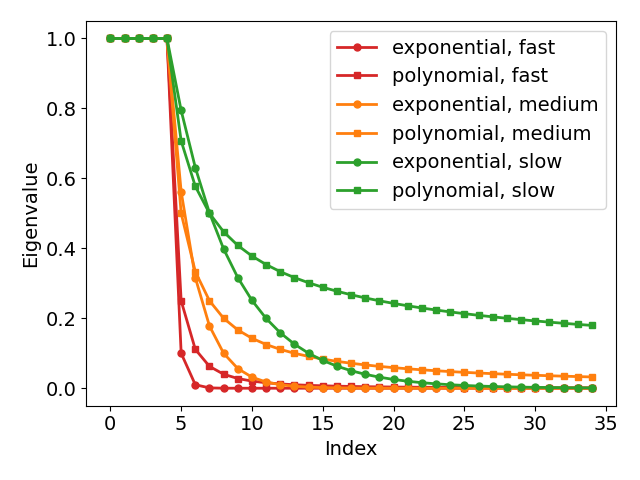
\includegraphics[width=0.45\textwidth]{synthetic_spectra.png}
		\hspace{0.02\textwidth} % Add horizontal space
		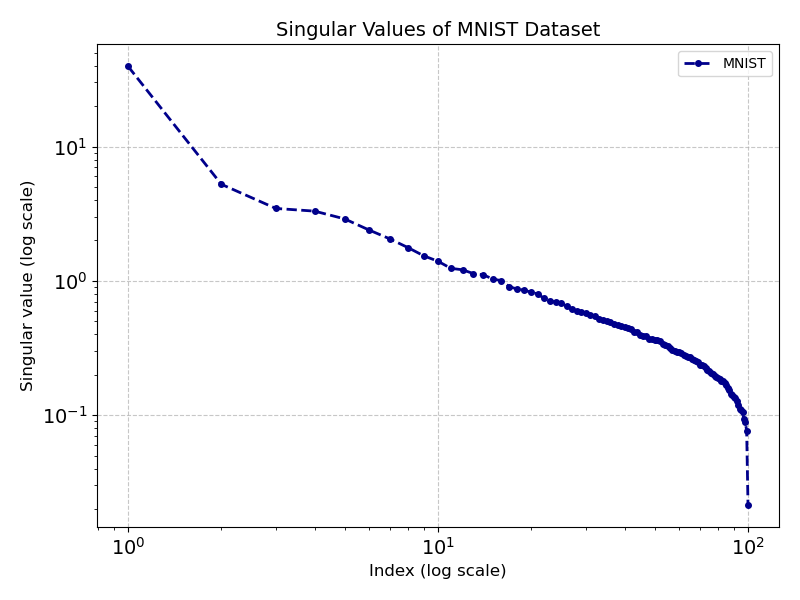
\includegraphics[width=0.45\textwidth]{mnist_singular_values_darkblue.png}
		\caption{Singular value decay of synthetic matrices (left) and the MNIST-based similarity matrix (right).}
		\label{fig:singular_value_comparison}
	\end{figure}
	\subsection{Stability Analysis}
	This section evaluates the numerical performance and stability of Gaussian Sketching and Block Subsampled Randomized Hadamard Transform (BSRHT) for low-rank matrix approximations. The trace-relative error, defined as 

	\begin{equation}
	\frac{\|A - A_{\text{approx}}\|_*}{\|A\|_*},
	\end{equation}
	
	where $\|\cdot\|_*$ represents the nuclear norm, is used to quantify the quality of the approximations. Smaller trace-relative error values indicate higher approximation quality. Additionally, the alignment of numerical results with theoretical guarantees established by the Oblivious Subspace Embedding (OSE) property is examined.
	
	The theoretical framework ensures that both Gaussian Sketching and BSRHT satisfy the $(\epsilon, \delta, d)$ OSE property. For Gaussian Sketching, the embedding dimension $l$ is given by:
	\begin{equation}
	l = \mathcal{O}\left(\epsilon^{-2}(d + \ln \frac{1}{\delta})\right),
	\end{equation}
	ensuring accurate approximations for any target rank $d$ with high probability. For BSRHT, the embedding dimension is:
	\begin{equation}
	l = \mathcal{O}\left(\epsilon^{-2}(d + \ln \frac{n}{\delta}) \ln \frac{d}{\delta}\right),
	\end{equation}
	making it scalable and efficient in distributed environments.
	
	Both methods conform to the following error bound:
	\begin{equation}
	\|A - A_{\text{approx}}\|_* \leq (1 + \epsilon) \|A - [[A]]_d\|_*,
	\end{equation}
	where $[[A]]_d$ is the optimal rank-$d$ approximation of $A$.

	\paragraph{Slow Exponential Decay:}

The results (Figure~\ref{fig:slow_fast_exp_decay}, left) show that Gaussian outperforms BSRHT Sketching for all ranks when $l$ is small (e.g., $l = 15$ or $l = 20$). 
As $l$ increases for example $l=170$ , we run into a problem :Tara fills . 


\paragraph{Fast Exponential Decay:}
For fast decaying spectra (Figure~\ref{fig:slow_fast_exp_decay}, right), Gaussian Sketching dominates at all ranks and embedding dimensions, showing superior accuracy. 
However, both Gaussian Sketching and BSRHT at $l=37$ display unexpected behavior, 
where the relative error does not decrease smoothly as expected for larger embedding 

\begin{figure}[H]
\centering
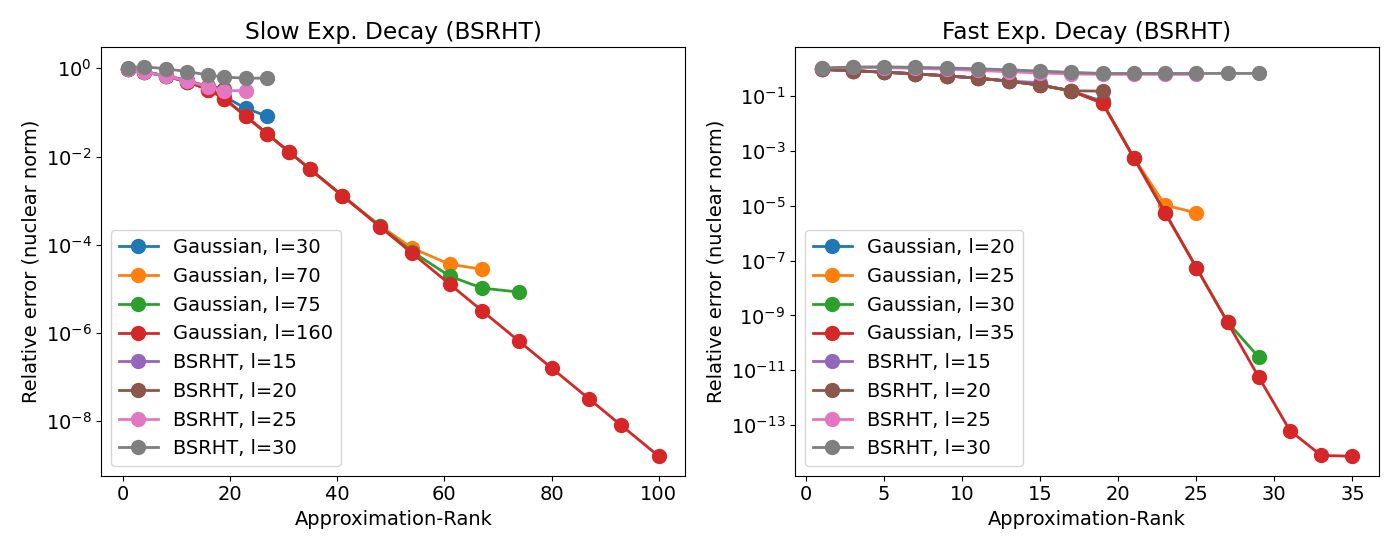
\includegraphics[width=0.975\textwidth]{exp_decay_stability_custom.png}
\caption{Relative error as a function of approximation-rank for different values of sketching dimension $l$ and both sketching methods. Dataset is taken as exponential (a) slowly-decaying and (b) fastly-decaying singular values.}
\label{fig:slow_fast_exp_decay}
\end{figure}

\paragraph{Slow Polynomial Decay:} 
For slow exponential decay (Figure~\ref{fig:poly_decay}, left), both Gaussian Sketching and BSRHT exhibit similar trends, with Gaussian Sketching showing slightly better performance. However, as \( l \) increases, their performance becomes nearly identical.

\paragraph{Fast Polynomial Decay:} 
n the fast polynomial decay scenario (Figure~\ref{fig:poly_decay}, right), Gaussian Sketching consistently outperforms BSRHT across all ranks and embedding dimensions. The relative errors for Gaussian Sketching decrease significantly as the rank increases, particularly for $l = 100$ and $l = 300$. In contrast, BSRHT shows a slower reduction in error, and its performance plateaus at higher ranks.
\begin{figure}[H]
\centering
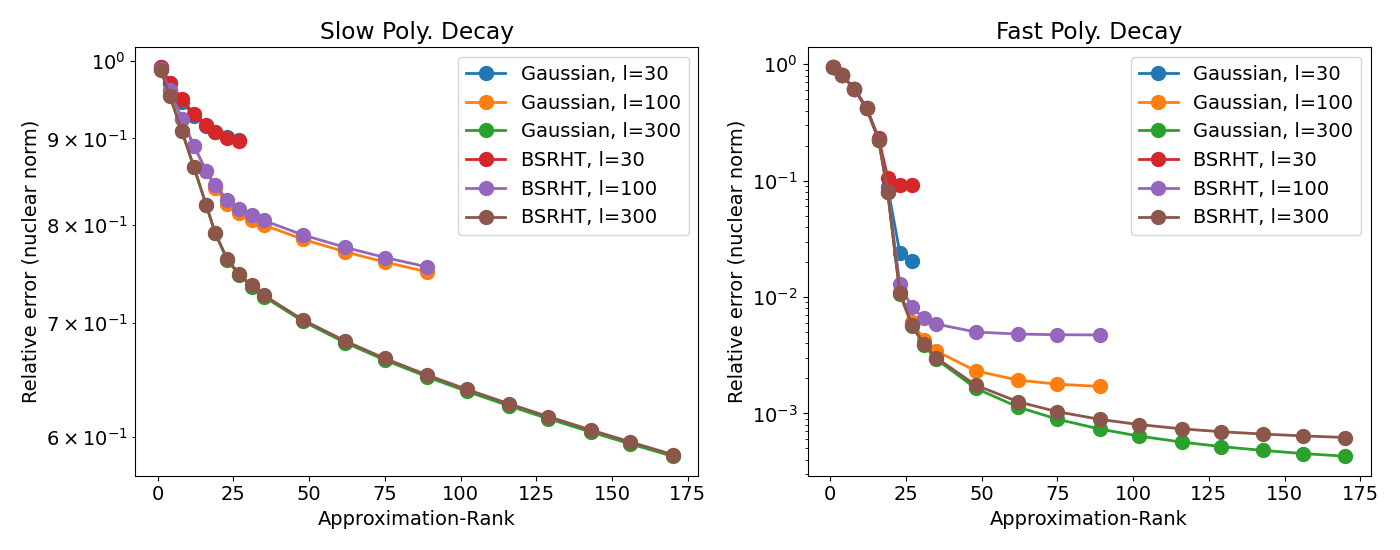
\includegraphics[width=0.975\textwidth]{poly_decay_stability_custom.png}
\caption{Relative error as a function of approximation-rank for different values of sketching dimension $l$ and both sketching methods. Dataset is taken as polynomial (a) slowly-decaying and (b) fastly-decaying singular values.}
\label{fig:poly_decay}
\end{figure}
\paragraph{MNIST}
The two methods exhibit almost identical behavior, with a minor difference at lower ranks, which completely disappears as the rank increases, as shown in Figure ~\ref{fig:mnsit_decay}.
\begin{figure}[H]
\centering
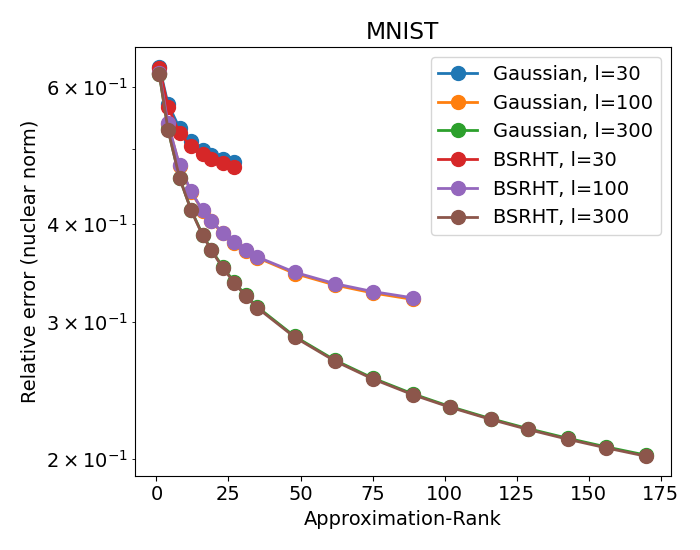
\includegraphics[width=0.45\textwidth]{MNIST_stability.png}
\caption{Relative error as a function of approximation-rank for different values of sketching dimension $l$ and both sketching methods. Dataset is taken as MNIST.}
\label{fig:mnsit_decay}
\end{figure}
	\subsection{Performance Analysis}
		For these results to have some general relevance, we tried considering realistic values of $k$ and $l$. More specifically, $k$ was taken often around $n/20$, while $l$ was taken logaritmically spaced.
	
		When running in parallel, the number of processors was limited to values $P=2^{2s}$ with $s\in\mathbb{N}$. This was due to perfect square constraint of the parallelised matrix multiplication and the BSRHT's use of the Hadamard transform. The values of $P$ we choose were 1,4,16,64. 		
		This also meant having to take $l\le n/64$ integer for the TSQR algorithm to not yield an error for $P=64$. We also recall that to see speed-up with TSQR we need the matrix to be tall-skinny. To have a good speed-up for a bigger $l$, while keeping numerical stability for ill-conditioned matrices another algo should be used.	

		Another implementation detail that should be mentioned is that we coded ourselves the Fast Hadamard Transform (starting from the python script on Wikipedia[4]). This was done to avoid using the only version we found online (from \texttt{simpy}), that was extremely slow. Details on the implementation can be found in the appendix \ref{apx:FWHT}.
		\section{Algorithm Performance}
        \subsection{Sequential Performance}
		To explore the sequential runtimes of the implemented algorithms, we decided to do two longitudinal studies : first varying $l$ for a selected value of $n$, and then varying $n$ for a selected $l$. The associated results are represented in \ref{fig:runtimes-l-n-variation}. 

		The main feature common to both plots is that the $k$ rank approximation part of the computation represents in most cases as small minority of runtime (as expected, since it should be of order $l^3 +nk^2$). This would of course change if one were to take big values of $k$ (i.e. if the data was really information-dense).  	
		It's runtimes also do not really seem to depend on the sketching method. This makes sense given the computations are the same regardless of which sketching method was used to obtain the $B$ and $C$ matrices. One could probably change this if one were to fully take advantage of the structure of the matrices involved in the BSRHT method (as one could use integer-float operations instead of float-float ones). 

		Looking more closely at both figures, it is clear that different behaviours are observed as a function of $l$ and $n$. We discuss each in the following paragraphs.
		\begin{figure}[htb]       
			\centering             
				\vspace{0em}
				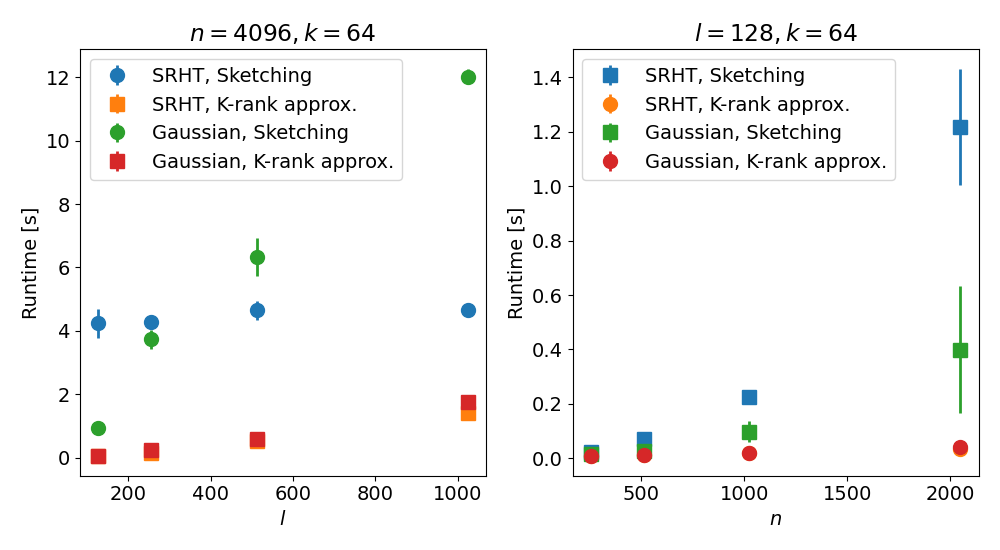
\includegraphics[width=.975\textwidth]{runtimes_l_n_variation}
				\caption{Runtimes associated to the tested sketching methods : as a function of $l$ (left) and as a function of $n$ (right). Runtimes are broken down in that associated to the computation of $A\Omega,\Omega^T A\Omega$ and that associated to the computation of the $k$ rank approximation.}
				\label{fig:runtimes-l-n-variation}
		\end{figure}
		\paragraph{$l$ variation}
		As a function of $l$ we observe extremely different behaviours from Gaussian and BSRHT sketchings. Indeed : the curve for BSRHT looks basically flat, while the Gaussian one increases steadily. This is expected given the complexities of the algorithms respectively are of order $n^2\log_2{n}$ and $nl^2 + ln^2$. This gives a great advantage in using BSRHT if we are embedding information-dense spaces as it scales much better.		

		Coming back to the $k$-rank approximation runtimes, we notice that the expected considerable increase as a function of $l$ is observed, even if as mentioned it stays relatively small when compared to the sketching runtime.
		\paragraph{$n$ variation}
		As a function of $n$ both algorithms show significant increase. BSRHT shows faster runtime growth. For $n=1024$ it seems to take twice the time, while for $n=2048$ it seems to take three times as much. This is a perfect match due to extra $\log_2(n)$ term in its complexity. This gives a considerable advantage in using Gaussian sketching when handling information-sparse within high dimensional spaces.

		As for the $k$-rank approximation runtimes, the linear increase as a function of $n$ is hard to see on the plot due to the different scale. 
        \subsection{Parallel Performance}
			We now turn to the analysis of the parallel performance. The relevant plot for this section is \ref{fig:runtimes-cores-variation}. 
			%For the sake of structure, we analyse separately the small and the large runs.
			\begin{figure}[htb]       
				\centering             
					\vspace{0em}
					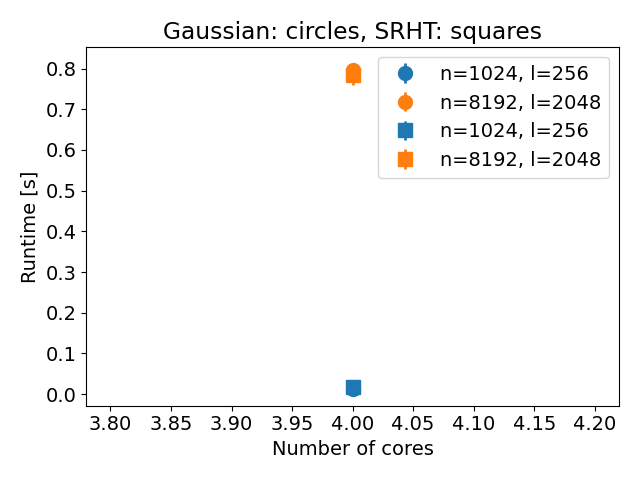
\includegraphics[width=.975\textwidth]{runtimes_cores_variation}
					\caption{Runtimes associated to the tested sketching methods as a function of the number of cores : for a ``small'' example (left) and a ``large'' one (right). Runtimes are broken down in that associated to the computation of $A\Omega,\Omega^T A\Omega$ and that associated to the computation of the $k$ rank approximation.}
					\label{fig:runtimes-cores-variation}
			\end{figure}
			%\paragraph{Small run}
			For the small run we first observe that some speed-up is displayed as a function of number of cores for both sketching methods. The speed-up is quasi-linear for BRSHT, while it saturates and back-fires for Gaussian sketching, due to the communication overhead. Given that the $k$-rank approximation part of the computation is smaller, it is most affected by the cost of communication, which actually dominates all throughout the core-number sweep.   
			These behaviours are expected given that : (a) the computation is rather small to be run in parallel; (b) BRSHT is slower than Gaussian sketching for small values of $l$. 
			
			For the specific parameter values selected, Gaussian sketching is a factor $\approx 10$ faster than BRSHT (except $P=64$).
			%\paragraph{Large run}
			For the large run the results are quite different. Communication is not an issue for the sketching part, meaning that quasi-linear speed-ups are observed for both methods. This means the parallelization is successful and scales well for big computations. We also observe initial speed-up for the $k$-rank approximation, though it is short-lived due to the computation still being quite small and due to that the matrix is not that tall-skinny (reducing the benefit in the QR decomposition). 
	\section{Conclusion}
	In this project, we studied the randomized Nystr\"om approximation algorithm for the low-rank approximation of a positive-semidefinite matrix $A \in \mathbb{R}^{n \times n}$. The goal was to efficiently parallelize this algorithm and investigate its numerical stability, scalability, performance (in terms of runtime), for both Gaussian and Block SRHT sketching methods and different decay patterns in $A$'s singular values. 
	
	The most important results for the performance side were that Gaussian sketching is faster than BSRHT for small values of $l$ and scales better with $n$, while BSRHT scales much better with $l$ making it a must for information-dense data. The parallelization was successful and scaled well for big computations. 
	
	In terms of stability, Gaussian sketching was found to be the most stable method, consistently outperforming BSRHT across various decay patterns for a fixed $l$. However, both methods showed irregular behaviors at certain embedding dimensions, which affected their performance. 
	
	Ultimately, choosing the method involves a trade-off between the mentioned stability and scalability properties, and should be tailored to the task and data at hand.
\newpage
	\section*{Appendix}
	\subsection*{Fast Walsh-Hadamard Transform}\label{apx:FWHT}
	We optimized the mentioned implementation of the FWHT in three ways. 
	
	Firstly, we removed the inner loop by operating on \texttt{i:i+h} directly. Then we removed copies of intermediate values by doing in-place computations. Finally, we adapted the function for it to act on matrices directly instead of a list of vectors (effectively replacing a \texttt{python} loop over the columns of $A$ with a \texttt{numpy} one).
	
	When analysing the resulting speed-up, we found it to be of around 3 (and therefore of around 30 compared to the \texttt{simpy} implementation). 
	\section*{Acknowledgements}
		\paragraph{Amal}
		ChatGPT was used to refine the English, generate code for the plots. Additionally, ChatGPT provided comments throughout the report and to the code to enhance readability.
		\paragraph{Tara}
		I personally use Github Copilot for coding purposes, as it can gain me some time by auto-completing lines. I however never keep lines I don't understand or find not relevant. I also sometimes used Chat GPT to brainstorm topics related to the debugging of the code.	
	\section*{References}
	[1] L. Grigori, ‘Randomized algorithms for low rank matrix approximation’.

	\noindent
	[2] ‘Algorithms’. Accessed: Dec. 26, 2024. [Online]. Available: \url{https://www.overleaf.com/learn/latex/Algorithms}

	\noindent
	[3] J. A. Tropp, A. Yurtsever, M. Udell, and V. Cevher, ‘Fixed-Rank Approximation of a Positive-Semidefinite Matrix from Streaming Data’.
	
	\noindent
	[4] ‘Fast Walsh–Hadamard transform - Wikiwand’. Accessed: Nov. 10, 2024. [Online]. Available: \url{https://www.wikiwand.com/en/articles/Fast%20Walsh%E2%80%93Hadamard%20transform}
	

	
%%%
\end{document} 